
\section{Consultar Tareas}

    Si el usuario da clic a la opción del menú \textit{Ver Tareas}
     
    \begin{figure}[H]
            \centering
            \hypertarget{VERT}{
\includegraphics[width=0.7\linewidth]{images/Tareas/Vertareaboton}}
            \caption{Opción Ver Tareas}
            \label{VERT}
    \end{figure}

    Se le redirecciona a la siguiente pantalla:
    \begin{figure}[H]
            \centering
            \hypertarget{asignart}{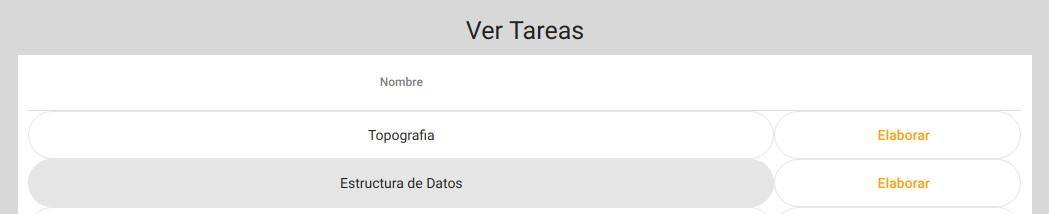
\includegraphics[width=0.7\linewidth]{images/Tareas/Vertareas}}
            \caption{Tabla de tareas}
            \label{asignart}
    \end{figure}
    Donde el usuario ve una tabla con todas las tareas relacionadas con él.